\documentclass{article}
\usepackage{hyperref}

\usepackage[utf8]{inputenc} %% Pour pouvoir utiliser les caractères accentués
\usepackage{graphicx} %% Pour pouvoir inclure des graphiques

\title{{\Huge \bf ENIB 2012 : S2P  MDD} \\
\vspace*{2cm}
{\Huge \bf Medius} \\----\\ Manuel utilisateur \\
\vspace*{2cm}
\centerline{
\includegraphics[height=3cm]{logomedius.jpg}}
}
\author{Valérian Saliou (v1saliou) \& Kwon-Young Choi (k1choi)}

%\date{La date}
\date\today 

\begin{document}
\maketitle

\newpage

\section{Introduction au jeu}

\subsection{Lancement du jeu}

Pour utiliser Medius, vous devez disposer de \begin{bfseries}Python\end{bfseries} (version 2.7 conseillée) avec \begin{bfseries}Pyglet\end{bfseries} (pour le jeu en lui-même) et \begin{bfseries}AVBin\end{bfseries} (pour le son).
\newline\newline
Une fois ces librairies installées, \begin{bfseries}ouvrez un terminal\end{bfseries}, puis entrez dans le répertoire de Medius (utilisez la commande cd).
\newline\newline
Enfin, exécutez \begin{bfseries}python main.py\end{bfseries} pour lancer le jeu.
\newline\newline

\subsection{Utilisation du jeu}

Medius a été conçu pour être relativement intuitif et simple d'utilisation.
\newline\newline
Au lancement du jeu, vous obtiendez le \begin{bfseries}menu général\end{bfseries} du jeu, vous permettant d'accéder à la liste des niveaux (bouton Jouer), de configurer votre jeu (cases à cocher) et d'obtenir quelques informations (bouton orné d'un i).
\newline\newline
Pour \begin{bfseries}lancer un niveau\end{bfseries}, cliquez sur Jouer. Vous arriverez dans l'écran de sélection de niveau. Vous avez à présent le choix entre bactérie et virus.
\newline\newline

\subsection{Prise en main du jeu}

Au cours du jeu, vous incarnerez un organisme qu'on appelle phagocyte. Le maniement se fait avec les flèches de votre clavier.
\newline\newline
Votre objectif est d'\begin{bfseries}enrayer l'infection\end{bfseries} bactérienne ou virale. Vous devez toucher les organismes étrangers (en vert) pour les éliminer.
\newline\newline
En parallèle, vous devez établir une stratégie pour empêcher la destruction totale de vos cellules (sur les côtés gauche et droit).
\newline\newline
Dans le cas général, les cellules et bactéries \begin{bfseries}se divisent aléatoirement\end{bfseries} par mitose.
\newline\newline
Les bactéries dégagent des projectiles (toxines) qui détruisent vos cellules et vous détruisent (vous réapparaissez alors au centre de la zone de jeu), tandis que les virus se servent de vos cellules pour se diviser en 3 après un court instant.
\newline\newline

\subsection{Aperçu du jeu}

\centerline{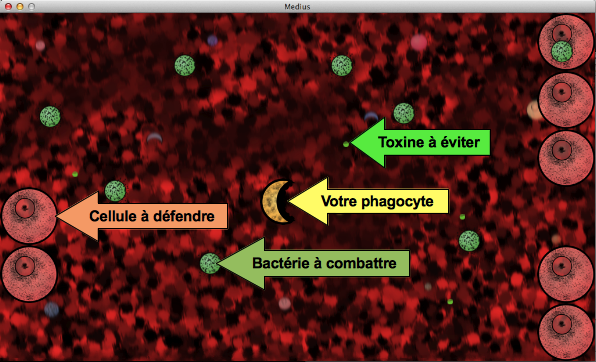
\includegraphics[height=7.5cm]{game_help.png}}
\strut\newline

\section{Progresser dans le jeu}

\subsection{Niveaux de difficulté}

Medius propose \begin{bfseries}3 niveaux de difficulté\end{bfseries} : du plus facile (1) au plus difficile (3).
\newline\newline
Le mode \begin{bfseries}facile\end{bfseries} (1) vous permet de comprendre le fonctionnement du jeu.
Le mode \begin{bfseries}intermédiaire\end{bfseries} (2) est accessible à tout joueur comprenant le jeu.
Le mode \begin{bfseries}difficile\end{bfseries} (3) vous demande de la stratégie, car il est impossible de gagner sans réflexion préalable sur votre méthode d'action.
\newline\newline

\subsection{Conseils de stratégies}

En mode difficile, vous devez \begin{bfseries}utiliser les rebonds\end{bfseries} sur les cellules latérales afin d'effectuer des changements de trajectoire rapides.
\newline\newline
Aussi, les organismes ennemis iront plus vite que votre phagocyte. Vous devrez donc les éliminer en les prenant à l'inverse de leur trajectoire, en arrivant face à eux.
\newline\newline
Évitez de passer à côté des cellules dans le cas des bactéries. En effet, celles-ci tirent \begin{bfseries}en votre direction\end{bfseries}, il est donc possible qu'un projectile atteigne une cellule qui se trouve derrière vous.
\newline\newline
Évitez que les virus dont une cellule est dans leur trajectoire ne l'atteigne, car celui-ci, en plus d'éliminer la cellule, s'en servira pour se diviser en 3.
\newline\newline

\section{Résoudre les problèmes}

\subsection{Je n'ai pas de son !}

Le \begin{bfseries}son est peut-être désactivé\end{bfseries} (vérifiez si les 2 cases sont cochées dans le menu général).
\newline\newline
Votre configuration ne peut peut-être pas lire le son. Veuillez \begin{bfseries}installer AVBin\end{bfseries}.
\newline\newline

\subsection{Mon jeu est lent !}

Votre ordinateur n'a peut-être pas suffisamment de \begin{bfseries}puissance disponible\end{bfseries}. Essayez de \begin{bfseries}fermer les applications\end{bfseries} consommatrices de ressources puis réessayez.
\newline\newline

\subsection{Je ne vois pas toute la fenêtre de jeu !}

Votre \begin{bfseries}résolution n'est pas suffisante\end{bfseries}. Medius requiert au moins une résolution de \begin{bfseries}1024x768\end{bfseries} afin d'être entièrement visible.
\newline\newline

\subsection{Mes paramètres ne sont pas sauvegardés !}

Medius ne doit pas avoir les \begin{bfseries}droits d'écriture\end{bfseries} dans sa base de donnée intégrée. Donnez les droits complets à tout utilisateur (\begin{bfseries}chmod 777\end{bfseries}) d'écrire et de lire sur le dossier ./db et son contenu.
\newline\newline

\section{Annexes}

\subsection{Développement du jeu}

Le \begin{bfseries}dépôt de développement\end{bfseries} de Medius est disponible sur Internet à l'adresse \begin{bfseries}\href{https://github.com/Vanaryon/medius}{https://github.com/Vanaryon/medius}\end{bfseries}
\newline\newline
Vous pouvez aussi y télécharger la dernière version du jeu.
\newline\newline

\end{document}